\documentclass[twocolumn]{article}

\usepackage{graphicx}
\usepackage{amsmath}
\usepackage{amsthm}
\usepackage{amssymb}
\usepackage{url}
\usepackage{multirow}
\usepackage{times}
%\usepackage{multicol}
\usepackage{fullpage}

\newcommand{\comment}[1]{}

\title{CS315: Group 23 \\
Real-time web portal for air pollution }
\author{
\begin{tabular}{ccc}
	Rachit Nimavat & Aniruddha Zalani & Balram Meena \\
	11466 & 11097 & 11189 \\
	%Roll Number 1 & Roll Number 2 & Roll Number 3 \\
	\url{nimavat@iitk.ac.in} & \url{aniruddh@iitk.ac.in} & \url{balram@iitk.ac.in} \\
	Dept. of CSE & Dept. of CSE & Dept. of CSE \\
	\multicolumn{3}{c}{Indian Institute of Technology, Kanpur}
\end{tabular}
}
\date{Final Report \\	% replace by ``initial'' or ``final'' as appropriate
17th April, 2014}	% replace by actual date of submission or \today

\begin{document}

\maketitle

\begin{abstract}
	%
Use of database management system for a real time air pollution monitoring is important for social, and more importantly enviornmental perpective. We have created \textbf{RAPID} - \textit{Realtime Air Pollution Index Daemon} for bringing about this awarness. The data generated by sensors installed in various parts of the world is collected by a central server which displays it instantaneusly on the website. Interface has been designed in such a way that it enables user to make a comparitive study between different cities and see the how hazardous is the current pollution level to health.
	%
\end{abstract}

\section{Introduction and Problem Statement}
Air pollution has become a major cause of concern due to rapid industrialiazation. The problem of air pollution is more acute in cities than in the country side. Therefore, it has become imperative to have a sytem that monitors air pollution and that is real time as well as reliable. Air pollution monitoring can help us understand how pollutants behave and their relationship with the weather. Monitoring data can be used to validate pollution modelling. Based on this data policies can be decided by the governments. Public can also benefit from easily available, accurate and up-to-date information on the quality of air. \\
\\
Objective of an air pollution monitoring system is to show accurate and real time data from the sensors installed in the cities, so that comparative studies can be made between different cities and countries.\\
We have considered around 1700 cities from all around the world for our project. 
\subsection{Problem statement}
\begin{itemize}
\item Collect data from incoming sensors at regular interval of time.
\item Insert data into the database taking care of consistency.
\item Reflect updated data on the webpage.
\item Give capability to the user to make different queries to analyse the data.
\subitem Display data on the world map.
\subitem Make charts and graphs to make comparision. 
\end{itemize}
\subsection{Related Material}
\begin{itemize}
\item \textbf{Data} was taken from data.gov.in. This data was inadequate for our analysis so on similar pattern we generated our own data.
\item \url{aqicn.org} is a real time pollution monitoring website of China. We looked towards it for ideas and checking the consistency of our generated data.
\item We have taken Sulplur Dioxide, Nitrogen Dioxide, Carbon Monoxide, Ozone, Respirable Suspended Particulate Matter (RSPM) and Fine Particulate Matter (FPM) as the indices of pollution.
\end{itemize}

\comment{

Can also comment out paragraphs, etc.

}
\section{Database Design}
\begin{figure}[t]
	\centering
	\hspace*{-1.8cm}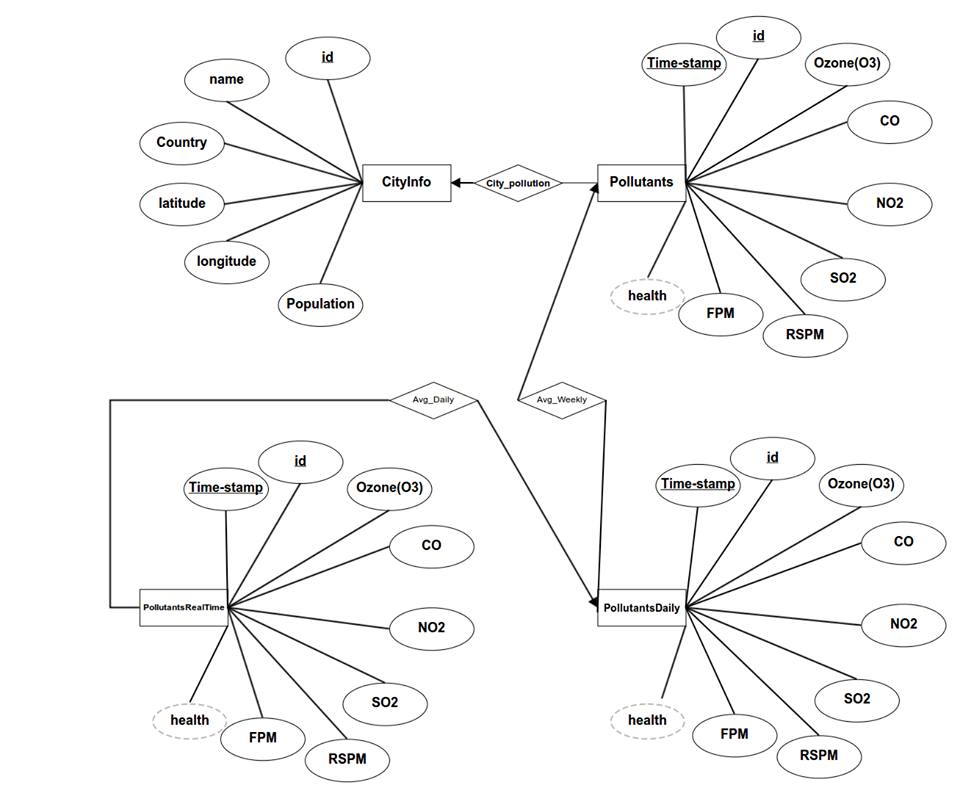
\includegraphics[width=1.2\columnwidth]{er2.jpg}
	\caption{ER Diagram}
	\label{fig:block}
\end{figure}
We have considered the scenario of managing portal for around 1700 polluted cities of the world. In real life scenario, there are 2-4 sample values of pollutant concentration available everyday \cite{cpcb}. This means, there would be less than 10,000 updates everyday. So, we have used MySQL as our database engine as it works excellent in these data ranges and is easy to  deploy \cite{mysql}. It would have been an overkill to use NoSQL or other database models.\\
\\
In our databse implementation, four tables have been made, \textbf{CityInfo} and \textbf{Pollutants} [Figure:\ref{fig:block}]. \textbf{CityInfo} contains the information of different cities of the world. It contains the location and demographic features of the city. Attributes named \textit{country, latitude, longitude} capture the location information a particular city and \textit{Population} reflects the demographic features. Primary key of the table is \textit{id} which is an auto-increment field.    \\ 
The \textbf{Pollutants} table has attributes for various indicators of pollution namely \textit{$SO_2$, $NO_2$, CO, $O_3$, RSPM, FPM}, derived attribute \textit{health}. Other attributes are  \textit{id} and \textit{time-stamp} which combined serve as primary key of the table.\\ The other two tables \textbf{PollutantsRealTime} and \textbf{PollutantsDaily} have same attributes as Pollutants table with the difference that the real time pollutants data from the sensors is first dumped into PollutantsRealTime whereas the AvgPollution table contains the daily average of different cities computed from PollutantsRealTime.
\subsection{Entity Relationship}
The tables in the database are related by the following relations - 
\begin{itemize}
\item The tables \textbf{Pollutants} and \textbf{CityInfo} are related via a many-to-one relation.  
\item The tables \textbf{Pollutants} and \textbf{PollutantsDaily} are related via a many-to-one relation.  
\item The tables \textbf{PollutantsDaily} and \textbf{PollutantsRealTime} are related via a many-to-one relation.  

\end{itemize}



\section{Approach}
\subsection{Data Generation}
The data \cite{gov} provided by the India Government was inadequate so on similar guidelines we generated data \cite{cpcb}. We assumed that the pollutants' concentration is  propotional to the population density. We generated the data as the Gaussian Distribution \cite{gauss} using this paramter as the mean and standard deviation to be propotional to square root of it. We found that this pattern most closely matches the data found on Centeral Pollution Control Board (CPCB) portal \cite{cpcb}.
\subsection{Data Update}
A main server was setup that collected data from the sensors (in our case client side). A cron job was set up that triggered the client side script at regular intervals. Data is sent over a TCP connection. This data is recieved by the server and inserted into the database. As soon as the data is recieved changes are being reflected on the website.\\
\\
For TCP connection a listening port is created at a server side which waits for the incoming connections and as soon as a connection is requested a new thread is created and which inserts new tuples into the database. Main challenge is to maintain the consistency of the database. For this changes were committed to the database only when the insert operation is successful otherwise changes are roll-backed. We used TCP as the mode of transferring data from clients to the server because it causes less network overhead at the server side and it is cheap to embed it into client pollution monitoring devices.

\subsection{Data Processing}
We set up a scheduled \textbf{event} in our database, firing up every month, to find the average pollution concentrations for the month for each city, and add that entry to a new table. Our aim was to make the generation of graphs on our portal fast and with less load on the server. By managing this new table, we could bring down query time close to 0.0 seconds, from around 0.5 seconds, with an additional one-time overhead of a fraction of the size.


\comment{

Use the following format for figures:

\begin{figure}[t]
	\centering
	\includegraphics[width=0.95\columnwidth]{figure_file}
	\caption{This figure explains this.}
	\label{fig:block}
\end{figure}

And refer as Figure \ref{fig:block}.

}

\subsection{Real Time Visualization}
As the data is sent over by the sensors over the TCP connection to the main server the data can be visualized over the webpage in real time. As soon as the data is recieved it is being dumped into \textbf{PollutantsRealTime} table and using Ajax\cite{ajax}, data is fetched from the database asynchronously, at every constant interval of time and then we plot the corresponding graph. 
\section{Results}
\subsection{Map}
	\begin{figure}[t]
	\centering 
	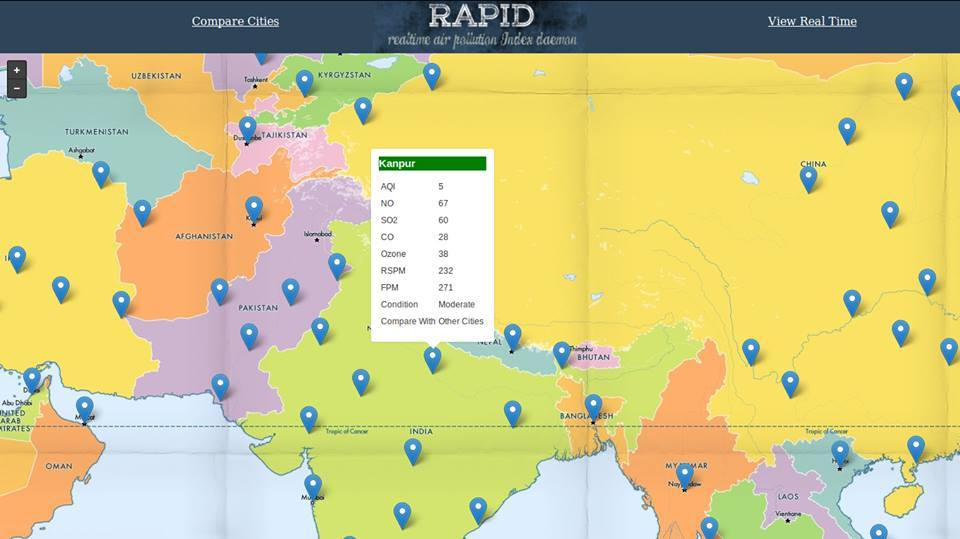
\includegraphics[width=0.95\columnwidth]{india.jpg} 
	\caption{UI for displaying the pollution concentrations} 
	\label{fig:kanpur} 
	\end{figure} 
	We have created a UI [Figure:\ref{fig:kanpur}] for displaying the pollution concentrations on the map, using an opensource tool MapBox \cite{mapbox}. We have added more UI features like exploring the monthwise pollution history of the place and comparing two cities on the same map. We also calculate the Air Pollution Index and colour-code the cities, based upon the concentration of our pollutant indices - viz, Sulplur Dioxide, Nitrogen Dioxide, Carbon Monoxide, Ozone, Respirable Suspended Particulate Matter (RSPM) and Fine Particulate Matter (FPM).\comment{

\begin{table}[t]
	\centering
	\begin{tabular}{|c||cc|}
		\hline
		Header 1 & Desc 1 & Desc 2 \\
		\hline
		\hline
		Row 1 & Data 1-1 & Data 1-2 \\
		Row 2 & Data 2-1 & Data 2-2 \\
		\hline
	\end{tabular}
	\caption{Table of results.}
	\label{tab:results}
\end{table}

And refer as Table \ref{tab:results}.

}
\subsection{Line Graphs}
Comparative studies can be done beween two cities [Figure:\ref{fig:compare}]. We have provided option to choose two cities from our database and the type of pollutants in our interface. Line graphs have been shown for the corresponding two cities where the X-axis represents the duration of time and Y-axis represents the concentration of pollutant.\\\\
\begin{figure}[t]
	\centering 
	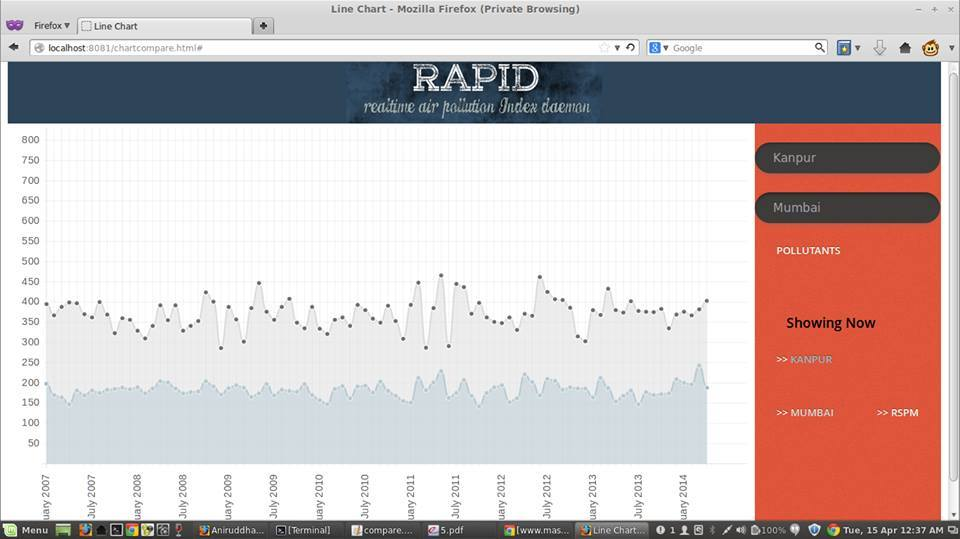
\includegraphics[width=0.95\columnwidth]{compare.jpg} 
	\caption{ Comapring the pollution concentrations for 2 cities} 
	\label{fig:compare} 
	\end{figure} 
\noindent
There is another option of \textbf{real time pollution analyser} for a city [Figure:\ref{fig:one}], where the data streamed by the sensors to the server is shown via a real time graph. 
\begin{figure}[t]
	\centering 
	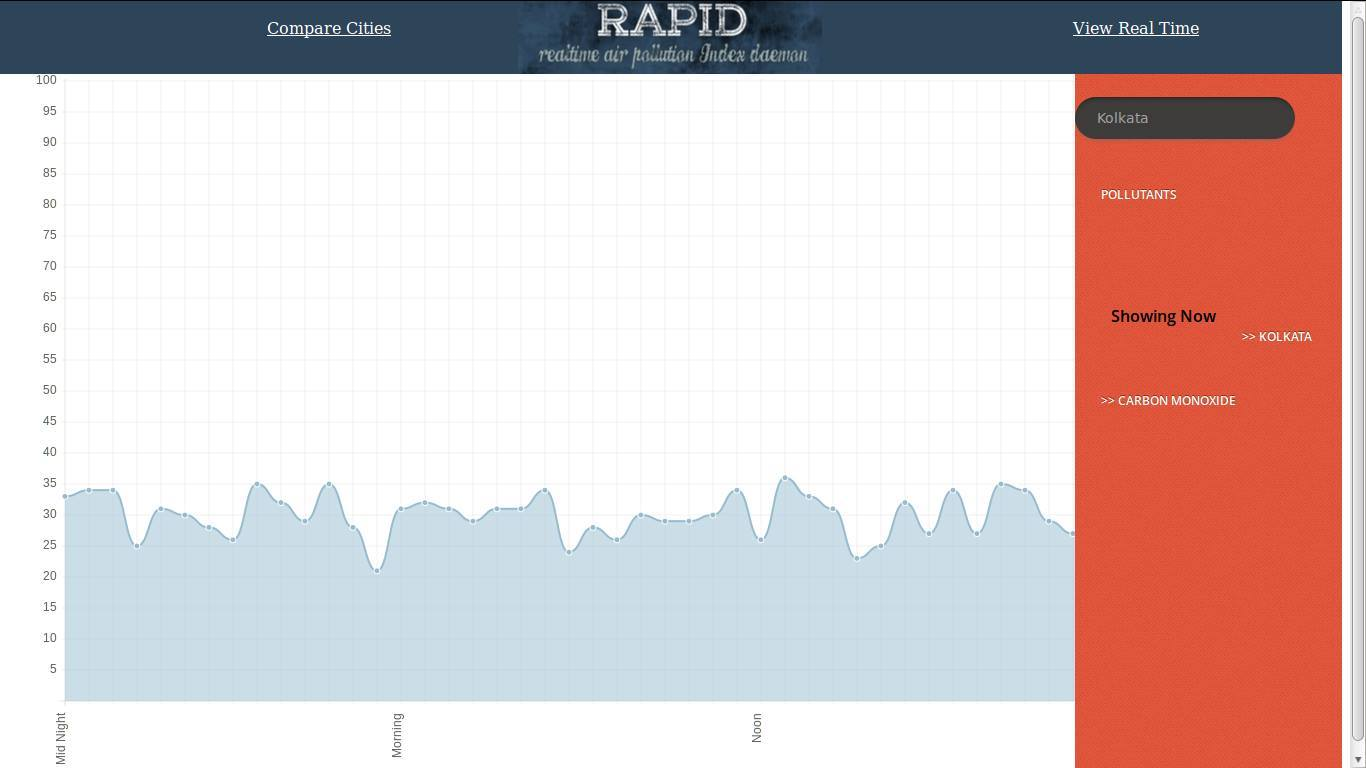
\includegraphics[width=0.95\columnwidth]{one.jpg} 
	\caption{Real Time pollution feed} 
	\label{fig:one} 
	\end{figure} 
\section{Conclusions}
Real time pollution monitoring system enables users to do comparitive study between different cities and also gives them index on the health hazards of the current pollution level. In the light of an increasingly large percentage of the population likely to experience increasingly severe adverse health effects, this knowledge and awarness is the key to precaution.

\section*{}
\begin{thebibliography}{2}
\bibitem{book} "Database System Concepts" by Silberschatz, Korth and Sudarshan. McGraw-Hill, Fifth Edition, 2006.
\bibitem{cpcb} Environmental Information System, Central Pollution Control Board, Ministry of Environment and Forests, Govt. of India. \textit{(http://cpcbenvis.nic.in/airpollution/database.htm)}
\bibitem{gauss} Gaussian Distribution, Wikipedia. \textit{(As on April 10, 2014)}
\bibitem{ajax} Ajax, Wikipedia \textit{(As on April 17, 2014)}
\bibitem{mapbox} MapBox on GitHub. \textit{https://github.com/mapbox}
\bibitem{gov} \textit{https://data.gov.in}
\bibitem{mysql} \textit{https://www.mysql.com/why-mysql/topreasons.html} 
\end{thebibliography}

\end{document}